\documentclass{article}
\usepackage[utf8]{inputenc}
\usepackage[spanish]{babel}
\usepackage{graphicx}
\usepackage{float}
\usepackage{pdfpages}
\usepackage{hyperref}
\usepackage{listings}
\graphicspath{{./img/}}


\definecolor{codegreen}{rgb}{0,0.6,0}
\definecolor{codegray}{rgb}{0.5,0.5,0.5}
\definecolor{codepurple}{rgb}{0.58,0,0.82}
\definecolor{backcolour}{rgb}{0.95,0.95,0.92}

\lstdefinestyle{mystyle}{
	backgroundcolor=\color{backcolour},   
	commentstyle=\color{codegreen},
	keywordstyle=\color{magenta},
	numberstyle=\tiny\color{codegray},
	stringstyle=\color{codepurple},
	basicstyle=\footnotesize,
	breakatwhitespace=false,         
	breaklines=true,                 
	captionpos=b,                    
	keepspaces=true,                 
	numbers=left,                    
	numbersep=5pt,                  
	showspaces=false,                
	showstringspaces=false,
	showtabs=false,                  
	tabsize=2
}
\lstset{style=mystyle}

\title{Práctica 3. Primera parte. Ingeniería de requisitos: Análisis y especificación de requisitos}
\author{Noelia Escalera Mejías\\
	\and Alejandro Menor Molinero\\
	\and Javier Núñez Suárez\\
	\and Adra Sánchez Ruiz\\
	\and Jesús Torres Sánchez}

\begin{document}
	\maketitle
	
	\section{Vecino más cercano}
	\subsection{Descripción}
	La primera heurística que usaremos es bastante sencilla: escogeremos una ciudad inicial y a partir de ahí seleccionaremos la ciudad más cercana a la última escogida (que no haya sido seleccionada previamente) hasta que no queden ciudades por añadir al circuito. Haremos varias ejecuciones, empezando cada vez de una ciudad distinta, y escogeremos la opción con distancia mínima.
	\begin{lstlisting}[caption=Pseudocódigo de la primera heurística, language=c]
	
	VecinosCercanos(distancias, n, resultado){
		completados;
		todas_las_ciudades;
		
		// Metemos los indices de las ciudades
		for (i=1; i<=n; i++)
			todas_las_ciudades.insert(i);
			
		// Iniciamos cada vez en una ciudad diferente
		for(i=1; i<=n; i++){
			candidatos = todas_las_ciudades;
			candidatos.erase(i);
			seleccionados.push_back(i);
			distancia = 0;
			
			//Creamos el circuito de la ciudad por la que empezamos
			while (!candidatos.empty()){
				actual = seleccionados.back();
				mas_cercano = *candidatos.begin();
				min = distancias[actual][mas_cercano];
				
				// Averiguamos la ciudad mas cercana
				for(c : candidatos){
					d = distancias[actual][c];
					if (d < min){
						mas_cercano = c;
						min = d;
					}
				}
				
				seleccionados.push_back(mas_cercano);
				distancia += min;
				candidatos.erase(mas_cercano);
			}
			distancia += (distancias[seleccionados.front()][seleccionados.back()]);
			
			completados[distancia] = seleccionados;
		}
		resultado = completados.begin()->second;
	}

	\end{lstlisting}
	\subsection{Resultados}
	\begin{figure}[H]
		\centering
		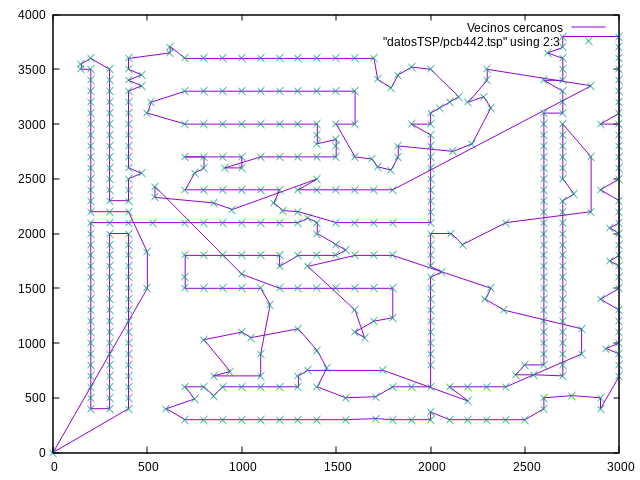
\includegraphics[totalheight=8cm]{img/vecinos_cercanos}
		\caption{Vecinos cercanos para tamaño 442}
		\label{fig:vecinos_cercanos}
	\end{figure}
\subsection{Eficiencia}
Este algoritmo es de orden $O(n^2)$, es bastante eficiente si tenemos en cuenta que en cada iteración hay menos ciudades entre las que hallar la ciudad más cercana. De todos los que analizaremos este es el más eficiente.
	\section{Inserción más económica}
	\subsection{Descripción}
	En este segundo algoritmo, empezamos con un circuito que contiene tres ciudades y posteriormente añadimos las ciudades restantes al recorrido. En cada iteración del algoritmo se busca la ciudad que tenga la inserción con menos coste en el circuito ya existente. Entendiendo como coste, la distancia que hay entre la ciudad a (ya existente) c (a insertar) más la distancia entre c y b(ya existente) menos la que hay entre a y b.
	
	\begin{lstlisting}[caption=Pseudocódigo de la segunda heurística, language=c]
		
		Insercion(distancias, n, resultado, ciudades){
			n = buscarCiudadNorte();
			s = buscarCiudadSur();
			e = buscarCiudadEste();
			
			resultado.aniade(n,s,e);
			distanciaFinal = distancias[n][e]+distancias[e][s]+distancias[s][n];
			
			for(int i=1;i<=n;i++){
				if(i!=n && i!=s && i!=e){
					candidates.insert(i);
				}
			}
			
			while(!candidatos.empty()){
				for(c:candidatos){
					for(it=resultado.begin(); it!=resultado.end();it++){
						siguiente = it;
						siguiente++;
						
						if(siguiente == resultado.end())
							siguiente = resultado.begin();
							
						diferencia = -distancias[*it][*siguiente];
						diferencia += distancias[*it][c];
						diferencia += distancias[c][*siguiente];
						
						 if (it == resultado.begin() || diferencia < distanciaMinima){
						distanciaMinima = diferencia;
						insercionMinima = it;
						}
					}
					if (distanciaMinima < calculoMinimo){
					calculoMinimo = distanciaMinima;
					posicionMinima = insercionMinima;
					candidataMinima = c;
					}
				}
				// Borramos de candidatos
				candidatos.erase(candidataMinima);
				
				// Insertamos 
				posicionMinima++;
				resultado.insert(posicionMinima, candidataMinima);
				
				// Actualizamos la distancia con la insercion
				distanciaFinal += calculoMinimo;
			}
			return distanciaFinal;
		}
	\end{lstlisting}
	\subsection{Resultados}
	\begin{figure}[H]
		\centering
		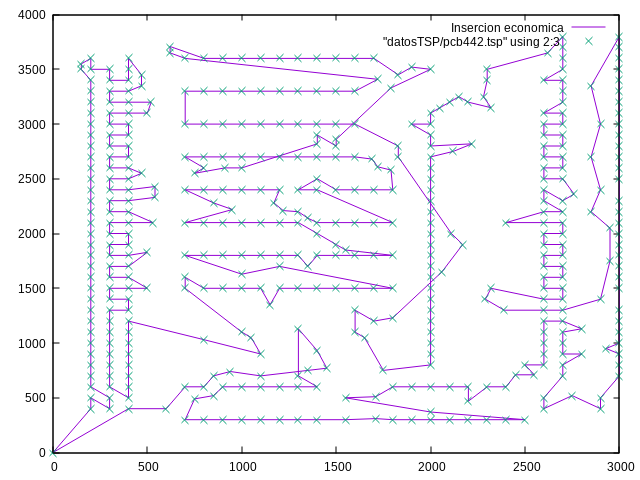
\includegraphics[totalheight=8cm]{img/insercion_economica}
		\caption{Inserción económica para tamaño 442}
		\label{fig:insercion_economica}
	\end{figure}
	\subsection{Eficiencia}
	Si bien la inserción económica representa en muchos casos una mejoría respecto a los vecinos cercanos en resultados, es peor en eficiencia. En este caso estamos hablando de un orden de $O(n^3)$
\section{Estrategia adicional}
	Hemos diseñado para este apartado dos algoritmos de inserción, la diferencia con respecto el segundo apartado es el circuito parcial del que partimos. Además de la eficiencia, (ambos son de orden $O(n^2)$)
	
	
	\
	
	En vez de elegir tres puntos (norte, sur y este), utilizamos el algoritmo de Jarvis para obtener la envolvente convexa, \textit{convex hull}, del conjunto de ciudades dadas. Este algoritmo pertenece al orden $O(n^2)$ de eficiencia.
	
	\
	
	Vamos a empezar definiendo qué es un \textbf{conjunto convexo}:
	
	\
	
	\textit{Un conjunto es convexo si dados dos puntos cualesquiera, el segmento que los une está contenido en el conjunto.} 
	
	\
	
\textit{	Una \textbf{envolvente convexa} es el menor conjunto convexo de un conjunto de puntos que los contiene.}
	
	\
	
	De esta envolvente convexa nos interesan las ciudades que hacen de límite para empezar con el circuito que forman, el algoritmo de inserción.
	
	\begin{figure}[H]
		\centering
		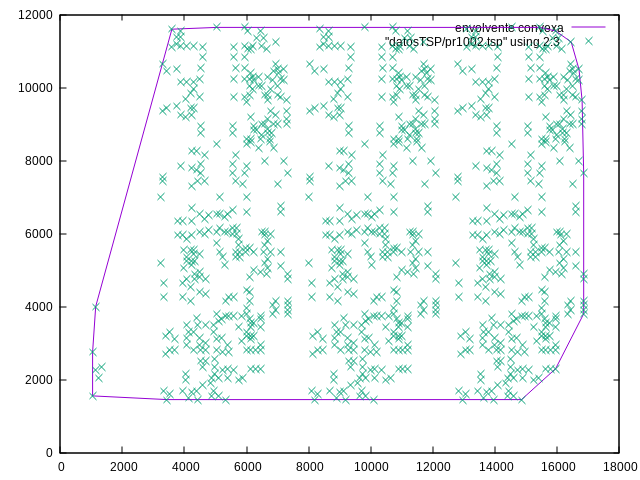
\includegraphics[totalheight=8cm]{img/envolvente_convexa}
		\caption{Envolvente convexa del conjunto de puntos pr1002.tsp}
		\label{fig:envolvente_convexa}
	\end{figure}
	\subsection{Inserción de la ciudad más lejana}
	Partiendo del circuito que acabamos de explicar, vamos a insertar ciudades del conjunto de candidatos (al principio las que no están en el circuito inicial) con la estrategia de insertar la ciudad más lejana respecto al conjunto de ciudades seleccionadas.
	
	\
	
	Es decir, primero iteramos por las seleccionadas para hallar la distancia a la que está la ciudad candidata de la ciudad mas lejana en el conjunto de seleccionadas.
	Después, de todas estas distancias, escogemos la mayor y la insertamos en el lugar más óptimo posible igual que en el segundo apartado.
	\begin{lstlisting}[language=c, caption =Pseudocódigo de inserción con envoltura convexa y ciudad más lejana]
	
	circuitoInicial = crearEnvolturaConvexa(ciudades)
	
	// Contiene todas las ciudades menos las que forman parte del circuito inicial
	candidatos = crear.conjunto()
	
	mientras(!candidatos.empty()){
		int ciudadMasLejana;
		int maximaDistancia;
		
		// Hallamos la ciudad mas lejana respecto
		// al conjunto de seleccionadas
		for (int c :candidatos){
			int dMasLejana;
			for (int s : seleccionadas){
				if (distancia(c,s) > dMasLejana)
					dMasLejana = distancia(c,s);
			}
			if (dMasLejana > maximaDistancia)
				ciudadMasLejana = c;
		}
		list<int>::iterator insercionMasBarata;
		int cuantoCuesta;
		
		for (auto it = resultado.begin() ; it != resultado.end() ; it++){
		auto siguiente = it;
		siguiente++;
		
		if (siguiente == resultado.end())
		siguiente = resultado.begin();
		
		int coste = -distancias[*it][*siguiente];
		
		coste += distancias[*it][ciudadMasLejana];
		coste += distancias[ciudadMasLejana][*siguiente];
		
		if (it == resultado.begin() || coste < cuantoCuesta){
			insercionMasBarata = it;
			cuantoCuesta = coste;
		}
		
		
		candidatos.erase(ciudadMasLejana);
		distancia += cuantoCuesta;
		insercionMasBarata++;
		resultado.insert(insercionMasBarata, ciudadMasLejana);	
	}
	return distancia;

	\end{lstlisting}
	
	\begin{figure}[H]
	\centering
	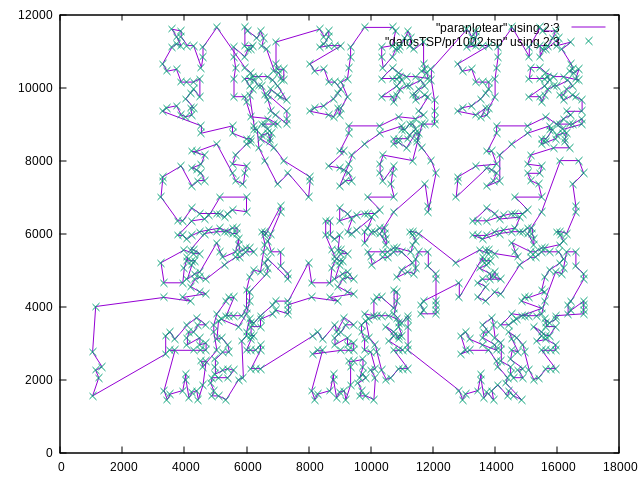
\includegraphics[totalheight=8cm]{img/convex_first}
	\caption{Resultado con estrategia de inserción ''mas lejana'' y partiendo de la envolvente convexa de pr1002.tsp}
	\label{fig:convex_first}
	\end{figure}
	\subsection{Inserción de la ciudad más cercana}
De nuevo partimos del circuito que hemos obtenido con la envolvente convexa, pero ahora vamos a escoger para la inserción la ciudad que más cerca esté del conjunto de seleccionadas.

\

Igual que antes, primero iteramos por las seleccionadas para hallar la distancia a la que está la ciudad candidata de la ciudad mas cercana en el conjunto de seleccionadas.
Después, de todas estas distancias, escogemos la menor y la insertamos en el lugar más óptimo posible igual que en el segundo apartado.
\begin{lstlisting}[language=c, caption =Pseudocódigo de inserción con envoltura convexa y ciudad más lejana]

circuitoInicial = crearEnvolturaConvexa(ciudades)

// Contiene todas las ciudades menos las que forman parte del circuito inicial
candidatos = crear.conjunto()

mientras(!candidatos.empty()){
int ciudadMasCercana;
int minimaDistancia = INT_MAX;

// Hallamos la ciudad mas cercana respecto
// al conjunto de seleccionadas
for (int c :candidatos){
int dMasCercana;
for (int s : seleccionadas){
if (distancia(c,s) < dMasCercana)
dMasCercana = distancia(c,s);
}
if (dMasCercana < minimaDistancia)
ciudadMasCercana = c;
}
list<int>::iterator insercionMasBarata;
int cuantoCuesta;

for (auto it = resultado.begin() ; it != resultado.end() ; it++){
auto siguiente = it;
siguiente++;

if (siguiente == resultado.end())
siguiente = resultado.begin();

int coste = -distancias[*it][*siguiente];

coste += distancias[*it][ciudadMasLejana];
coste += distancias[ciudadMasLejana][*siguiente];

if (it == resultado.begin() || coste < cuantoCuesta){
insercionMasBarata = it;
cuantoCuesta = coste;
}


candidatos.erase(ciudadMasLejana);
distancia += cuantoCuesta;
insercionMasBarata++;
resultado.insert(insercionMasBarata, ciudadMasLejana);	
}
return distancia;

\end{lstlisting}

\begin{figure}[H]
	\centering
	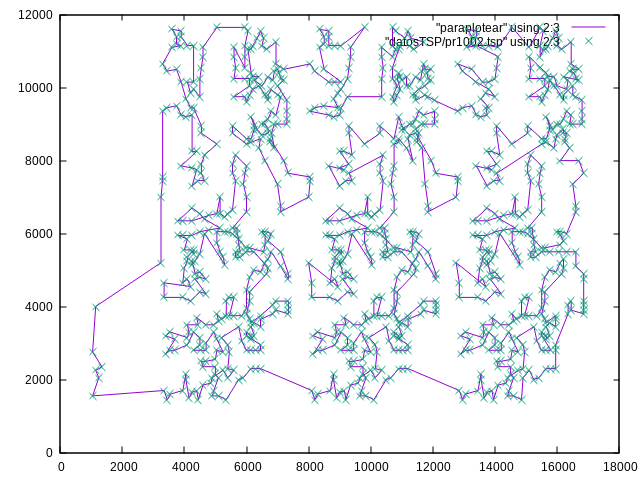
\includegraphics[totalheight=8cm]{img/convex_second}
	\caption{Resultado con estrategia de inserción ''más cercana'' y partiendo de la envolvente convexa de pr1002.tsp}
	\label{fig:convex_second}
	\end{figure}	


\section{Comparativa final y conclusiones}
A continuación, hemos realizado una comparativa con las soluciones para cada una de las 4 versiones. Para ello, hemos ejecutado los algoritmos a partir de una serie de mapas y, para cada distancia calculada de cada algoritmo, hemos obtenido el \textbf{cociente comparativo} entre la distancia obtenida y la distancia óptima (datos ya proporcionados).\\
Tras realizar este estudio, podemos observar los siguientes resultados:
\begin{figure}[H]
	\centering
	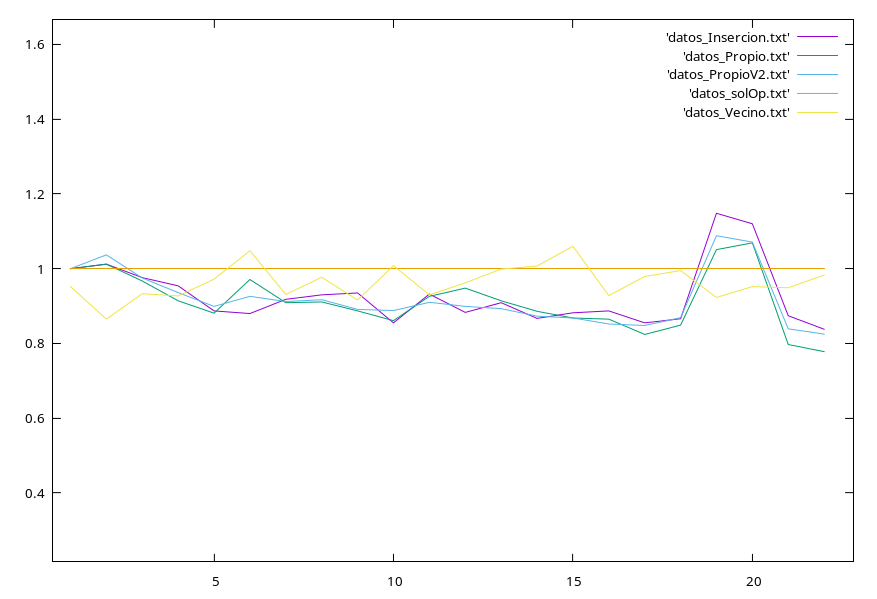
\includegraphics[totalheight=6cm]{img/comparativa}
	\caption{Gráfica comparativa de resultados}
	\label{fig:comparativa}
\end{figure}

Como conclusión, podemos observar como, aunque en general el algoritmo basado en la selección del vecino más cercano parece el más óptimo, no podemos afirmar que lo sea. Dependiendo del mapa obtenemos resultados muy variados; en algunos destaca el algoritmo del vecino, pero en muchos otros es menos óptimo que el resto. Esto ocurre debido a que la optimalidad de nuestros algoritmos no solo depende del tamaño del problema, sino que también depende de otros factores como la disposición de las ciudades en el mapa.

 \

Finalmente, para tener una visión más amplia de los resultados generados por nuestros algoritmos, podemos observar los resultados para un mapa sencillo (22 ciudades):

\begin{figure}[H]
	\centering
	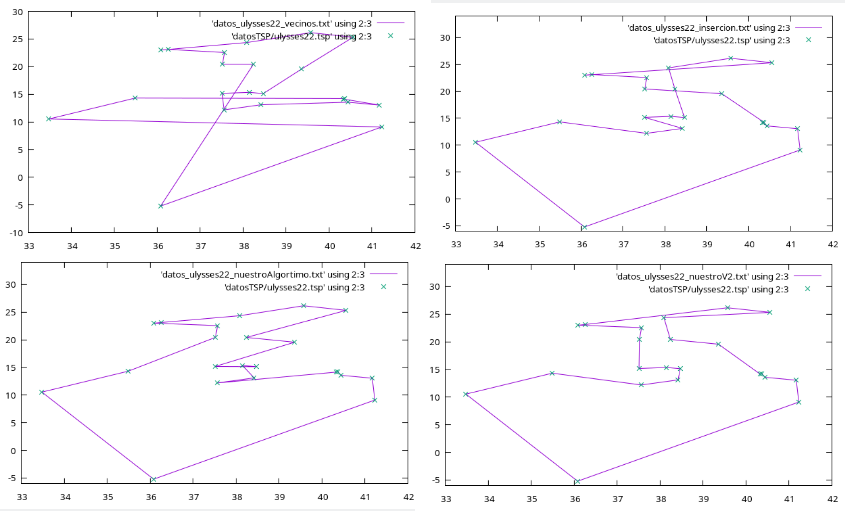
\includegraphics[totalheight=8cm]{img/comparativa3}
	\caption{Comparativa con el ejemplo de 22 ciudades}
	\label{fig:comparativa3}
\end{figure}



\section{Fuentes}
Para acabar mencionar brévemente de dónde nos hemos informado para implementar los algoritmos del apartado 3:
\begin{itemize}
 \item \href{https://en.wikipedia.org/wiki/Convex_hull}{Página de wikipedia sobre la envoltura convexa}
 \item \href{https://ocw.mit.edu/courses/civil-and-environmental-engineering/1-203j-logistical-and-transportation-planning-methods-fall-2006/lecture-notes/lec16.pdf}{MIT Open Course Ware sobre heurísticas del TSP}
 \item \href{https://en.wikipedia.org/wiki/Gift_wrapping_algorithm}{Página de la wikipedia sobre el algoritmo de Jarvis}
\end{itemize}

\end{document}